%%%% fs-run-time-experiments   Experiments

\label{fs-experiments-section}

We performed the series of experiments to estimate the performance of our system's prototype. As a stream processing task, we apply building an inverted index. This task is chosen because it has the following properties:

\begin{enumerate}
    \item Task requires stateful operations. It allows us to check the performance of the proposed stateful pipeline
    \item Computational flow of the task contains network shuffle that can violate the ordering constraints of some operations. Therefore, inverted index task can verify the performance of our optimistic approach
\end{enumerate}

It is worthwhile to mention that building inverted index can be considered as the halfway task between documents generation and searching. In the real-world, such scenario can be found in freshness-aware systems, e.g., news processing engines.

Building of inverted index is implemented in terms of MapReduce transformations. We start with page mapping into the pairs {\it (word; word positions within the page)}. After that, word positions are reduced by word into the single structure. We assume the output of the stream to be change records of the inverted index structure, i.e., each input page triggers the output of the corresponding updates. 

Pairs {\it (word; word positions within the page)} must be ordered by page id and version before the update of inverted index state. Otherwise, it is possible to obtain the inconsistent index, if there are multiple versions of the same document.  
 
In \FlameStream\ this algorithm is implemented as the typical conversion of MapReduce transformation, which is shown in section~\ref{fs-drifting}. Inverted index structure plays the role of an accumulator, and the accumulator map produces the most recent changes of this structure if any.

By the notion of {\it latency} we assume the time between two events: 

\begin{enumerate}
    \item Input page is taken into the stream
    \item All the change records for the page leave the stream
\end{enumerate}

Our experiments were performed on the cluster of Amazon EC2 micro instances with 1GB RAM and 1 core CPU. We used 10000 Wikipedia articles as a dataset. 

\subsection{Overhead and scalability}
The proposed method can bring an additional overhead. Thus, it is essential to analyze the system's behavior under different configurations.

We take the ratio of arrived at the barrier items count to the number of the valid items among them as a key metric for the estimation of the overhead of our prototype. This value measures the extra cost of our approach.

The relation between the number of workers, the input document's average rate, and the proposed ratio is shown in Figure~\ref{overhead}. As expected, the peak of the ratio is achieved when the document per second rate is high, and the number of the nodes is low. This behavior can be explained by the fact that a few workers cannot effectively deal with such intensive load. Nevertheless, the proportion of invalid items reduces with the increase of workers number. Under not very high pressure, the total overhead of the optimistic approach is under 10\% for all considered number of workers. These results confirm that the ratio does not increase with the growth of the number of nodes.

\begin{figure}[ht]
  \centering
  \begin{minipage}[b]{.6\textwidth}
    \centering
    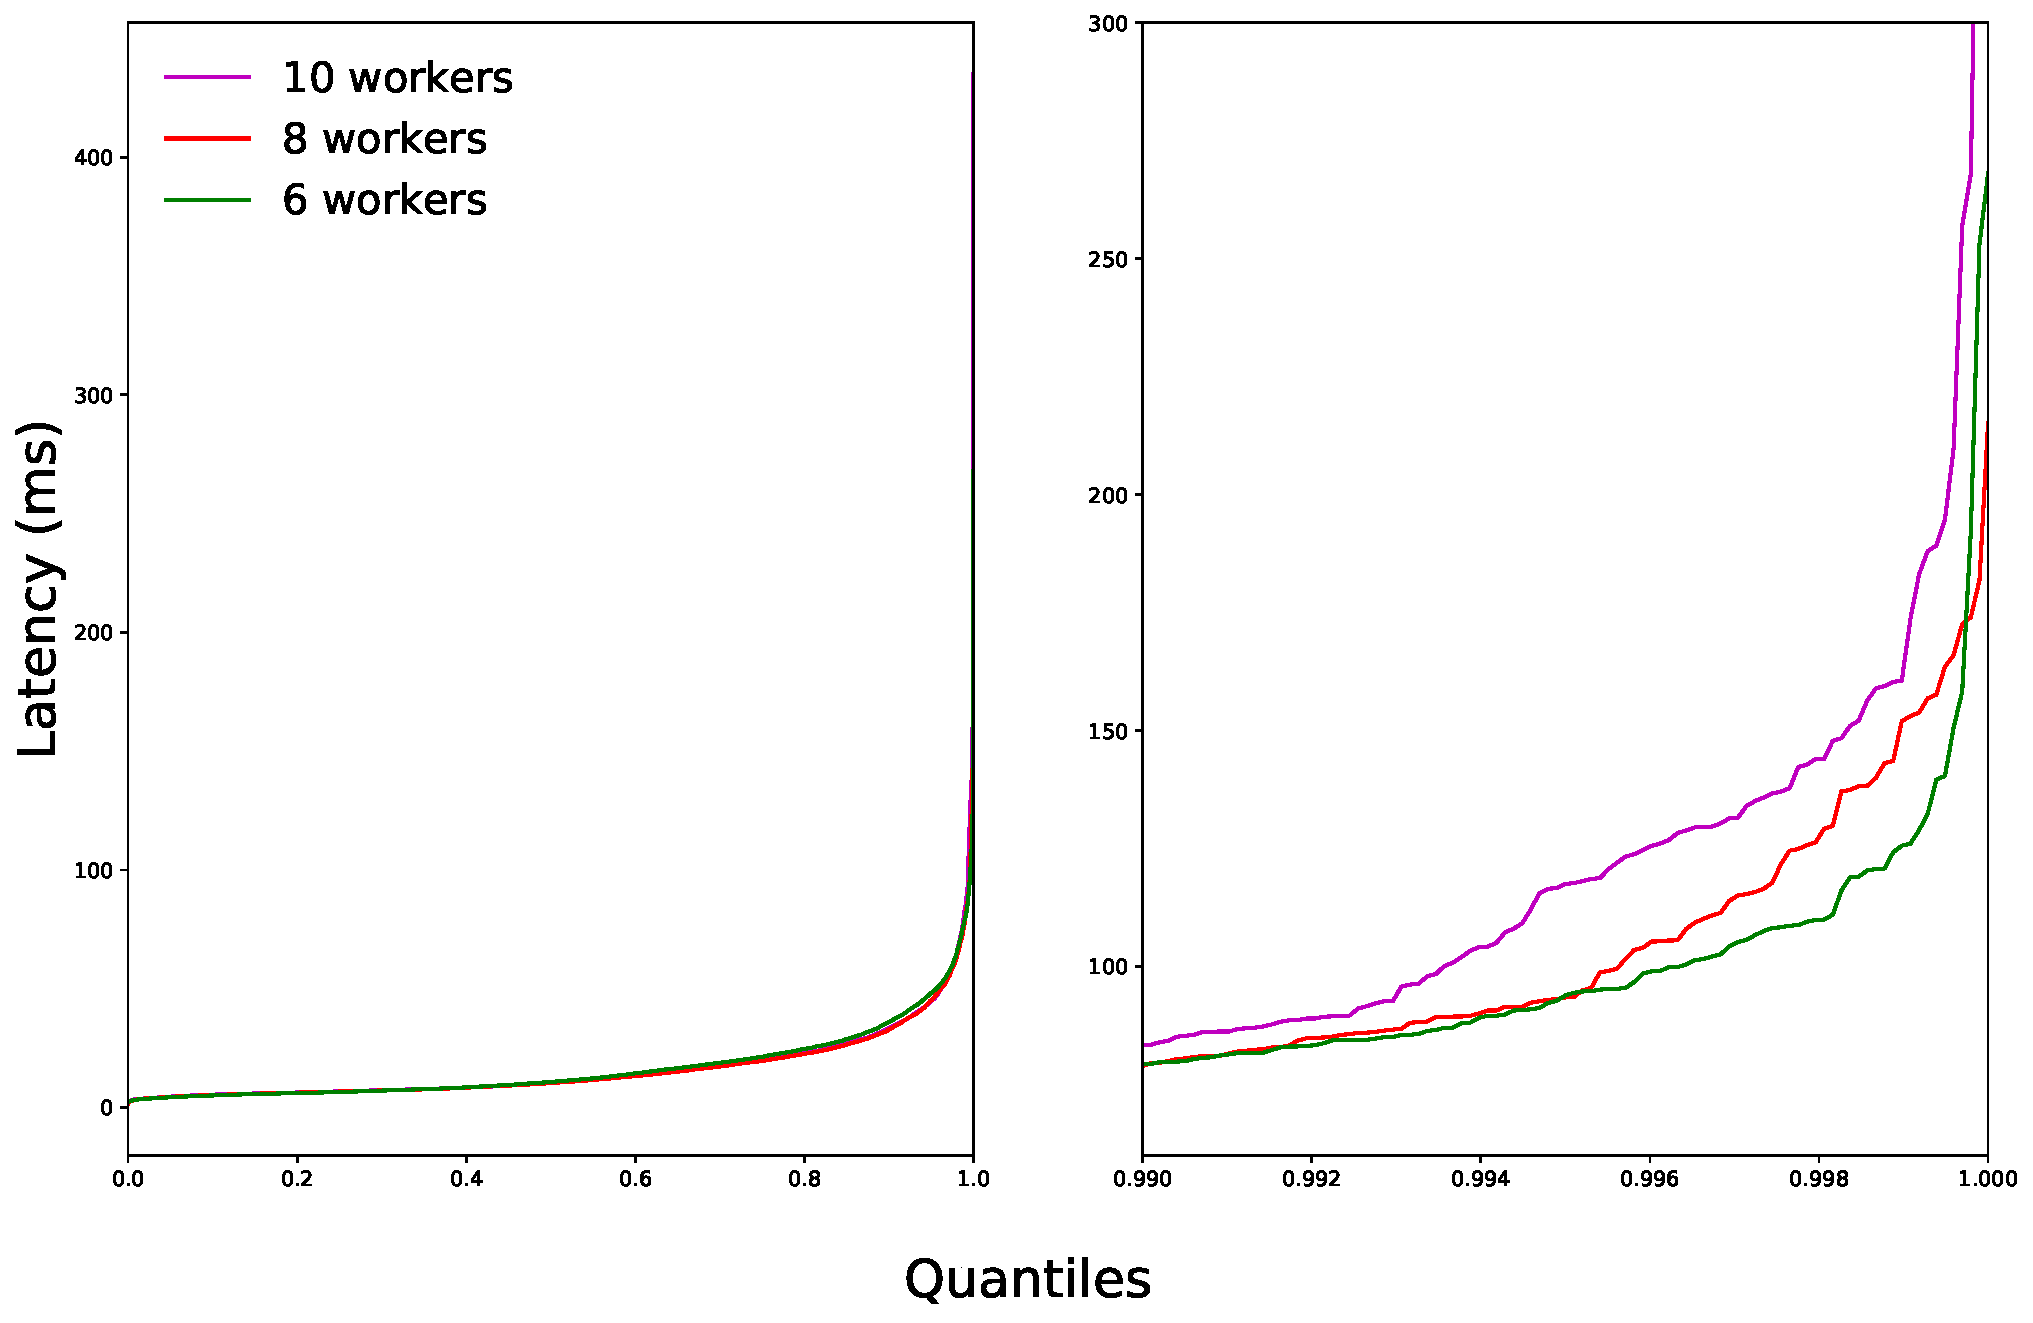
\includegraphics[width=\linewidth]{pics/fs-index-quantiles}
    \caption{FlameStream latency distribution. Left - the whole distribution, right - high quantiles}
    \label{fs-index-quantiles}
  \end{minipage}%
  \begin{minipage}[b]{.40\textwidth}
    \centering
    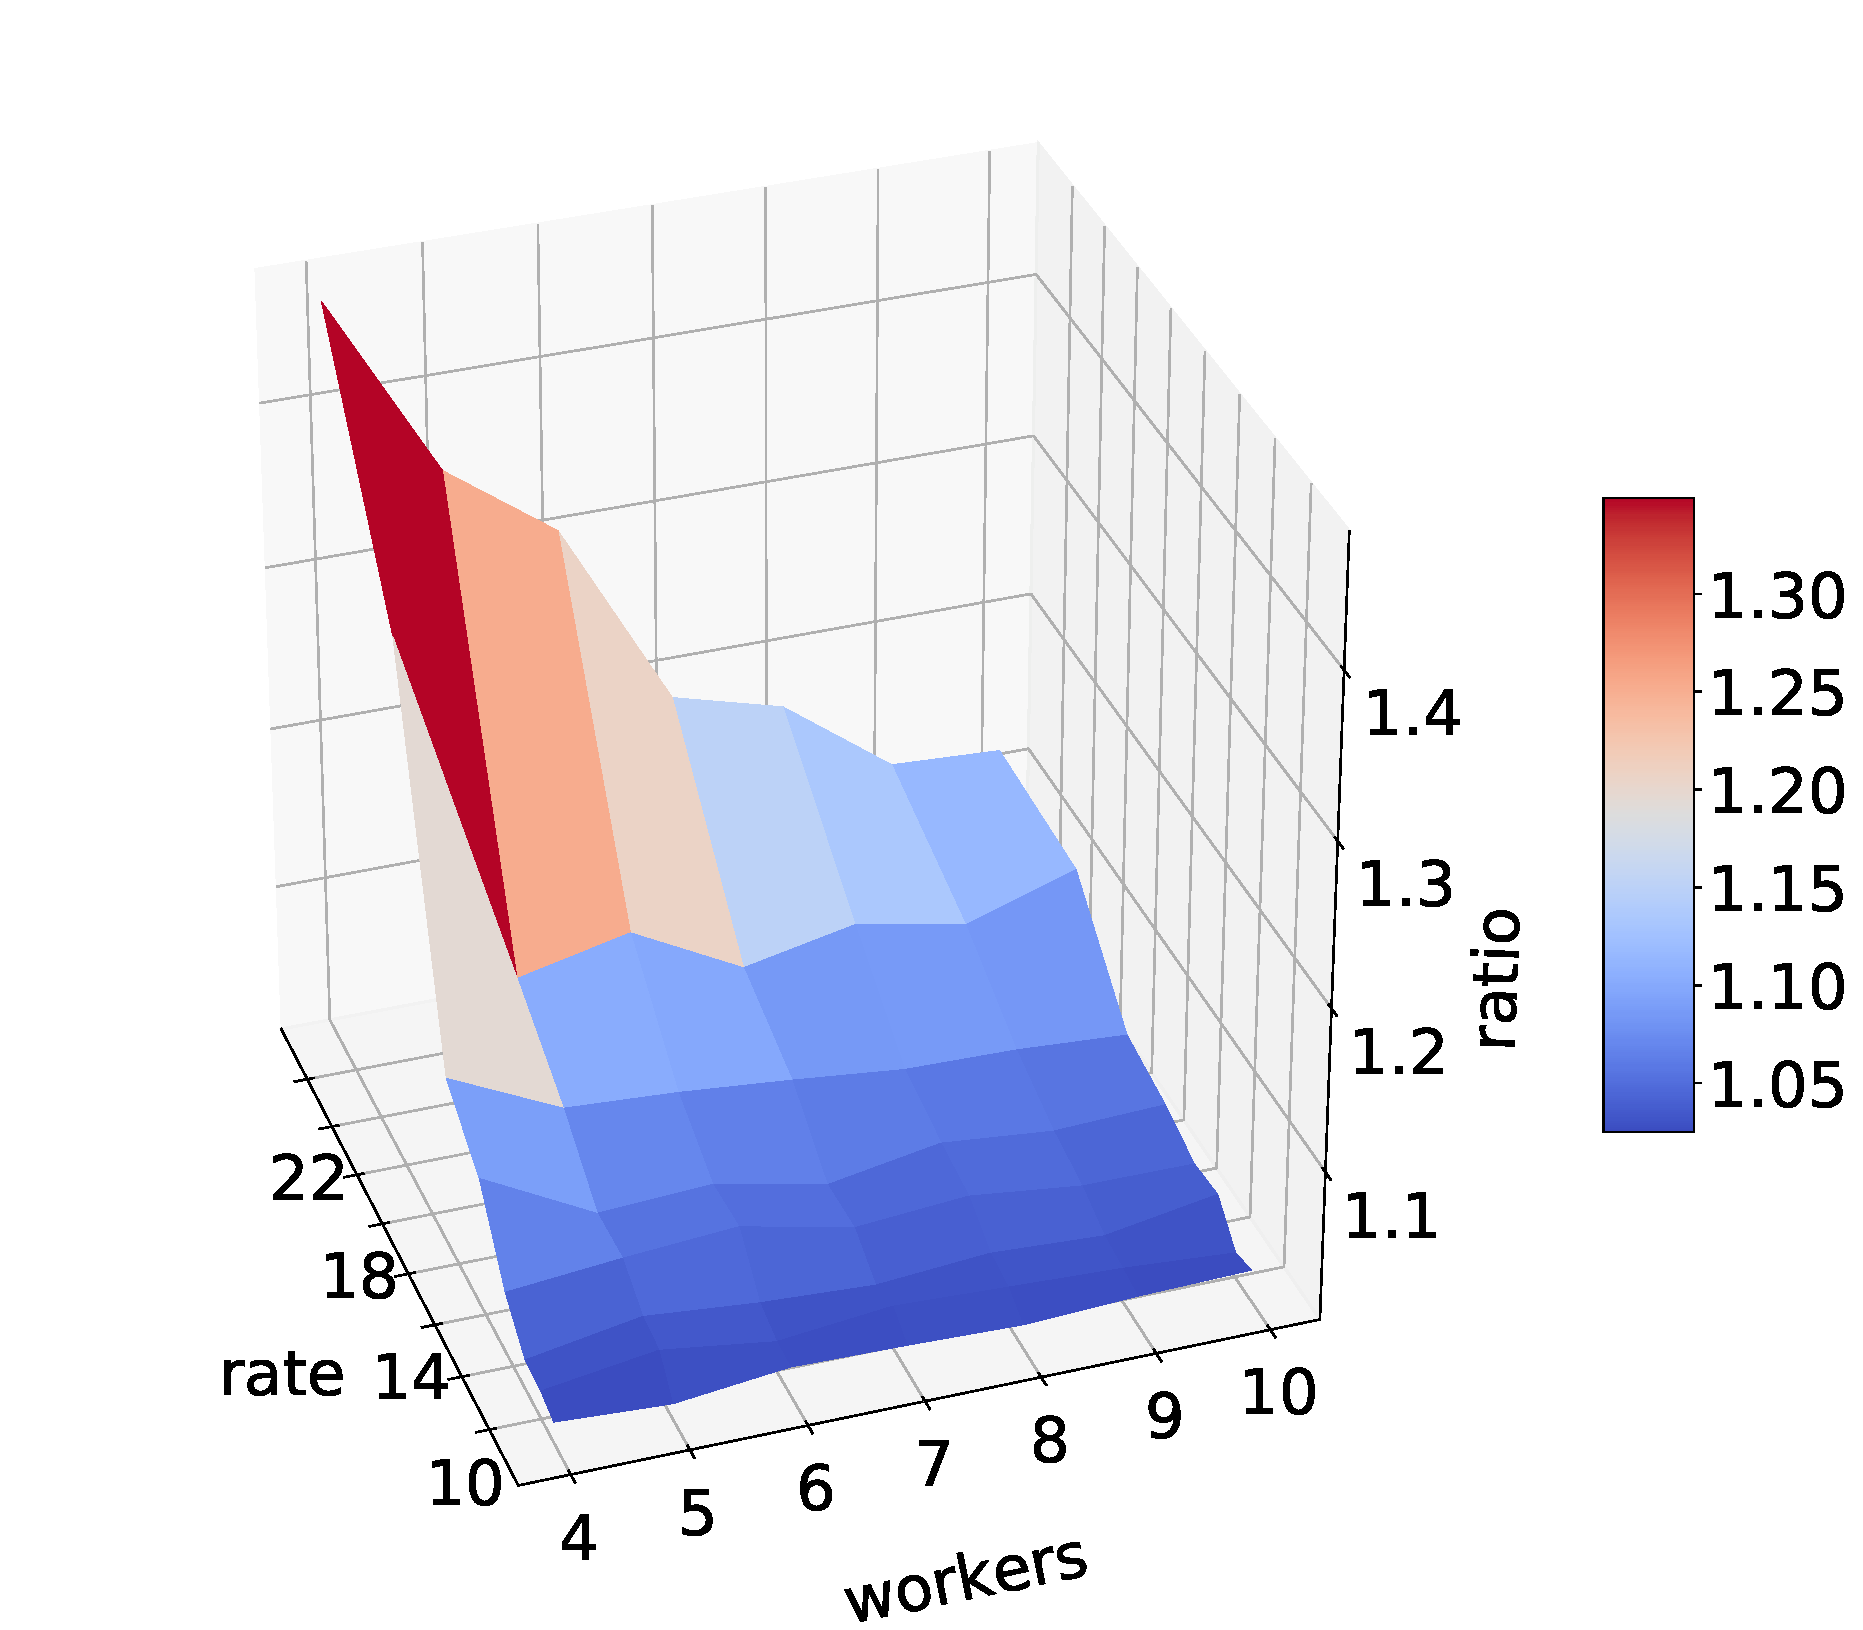
\includegraphics[width=\linewidth]{pics/overhead}
    \caption{The relation between the number of workers, the input document's average rate and the repair ratio}
    \label{overhead}
  \end{minipage}%
\end{figure}

The latencies of \FlameStream\ across multiple workers for the fixed document rate of 70 ms are shown in Figure~\ref{fs-index-quantiles}. This figure demonstrates that latency is not significantly increased with the growth of the number of workers. 

Therefore, the most important conclusions of these experiments are: the proposed method is scalable, the overhead could be optimized by system setup.

\subsection{Comparison against Apache Flink}

One of the most important goals of the experiments is the performance comparison with an industrial solution regarding latency. Apache Flink is chosen for evaluation because it is state-of-the-art stream processing system that provides similar functionality and achieves low latency in the real-world scenarios~\cite{S7530084}. 

For Apache Flink, the algorithm for building the inverted index is adopted by the usage of {\it FlatMapFunction} for map step and stateful {\it RichMapFunction} for reduce step and for producing the change records. Order enforcing before reduce is implemented using custom {\it ProcessFunction} that buffers all input until corresponding low watermark is received. Watermarks are sent after each document. The network buffer timeout is set to 0 to minimize latency.

In this paper, we compare $50^{th}$, $75^{th}$, $95^{th}$, and $99^{th}$ percentile of distributions, which clearly represent the performance from the perspective of the users' experience.

The comparison of latencies between \FlameStream\ and Flink within 10 nodes and distinct document rates is shown in the (a) plot in Figure~\ref{fs-index-quantiles}. In this case, \FlameStream\ provides lower latency even under high load. These results confirm that optimistic approach for deterministic processing is able to provide less latency than conservative methods. Firstly, the reason for better performance can be the fact that Flink starts to update index only after the buffer before reduce stage is flushed. In contrast, \FlameStream\ flushes its barrier right before data is sent to a user, according to its optimistic nature. At this moment, all corresponding computations have been already done. Secondly, low watermarks go along the stream and can be delayed by long-running operations, while acker processes ack messages independently. It is confirmed by (c) plot in Figure~\ref{fs-index-quantiles}, which shows the comparison between waiting time in Flink buffer and \FlameStream barrier.

\begin{figure}[ht]
  \centering
  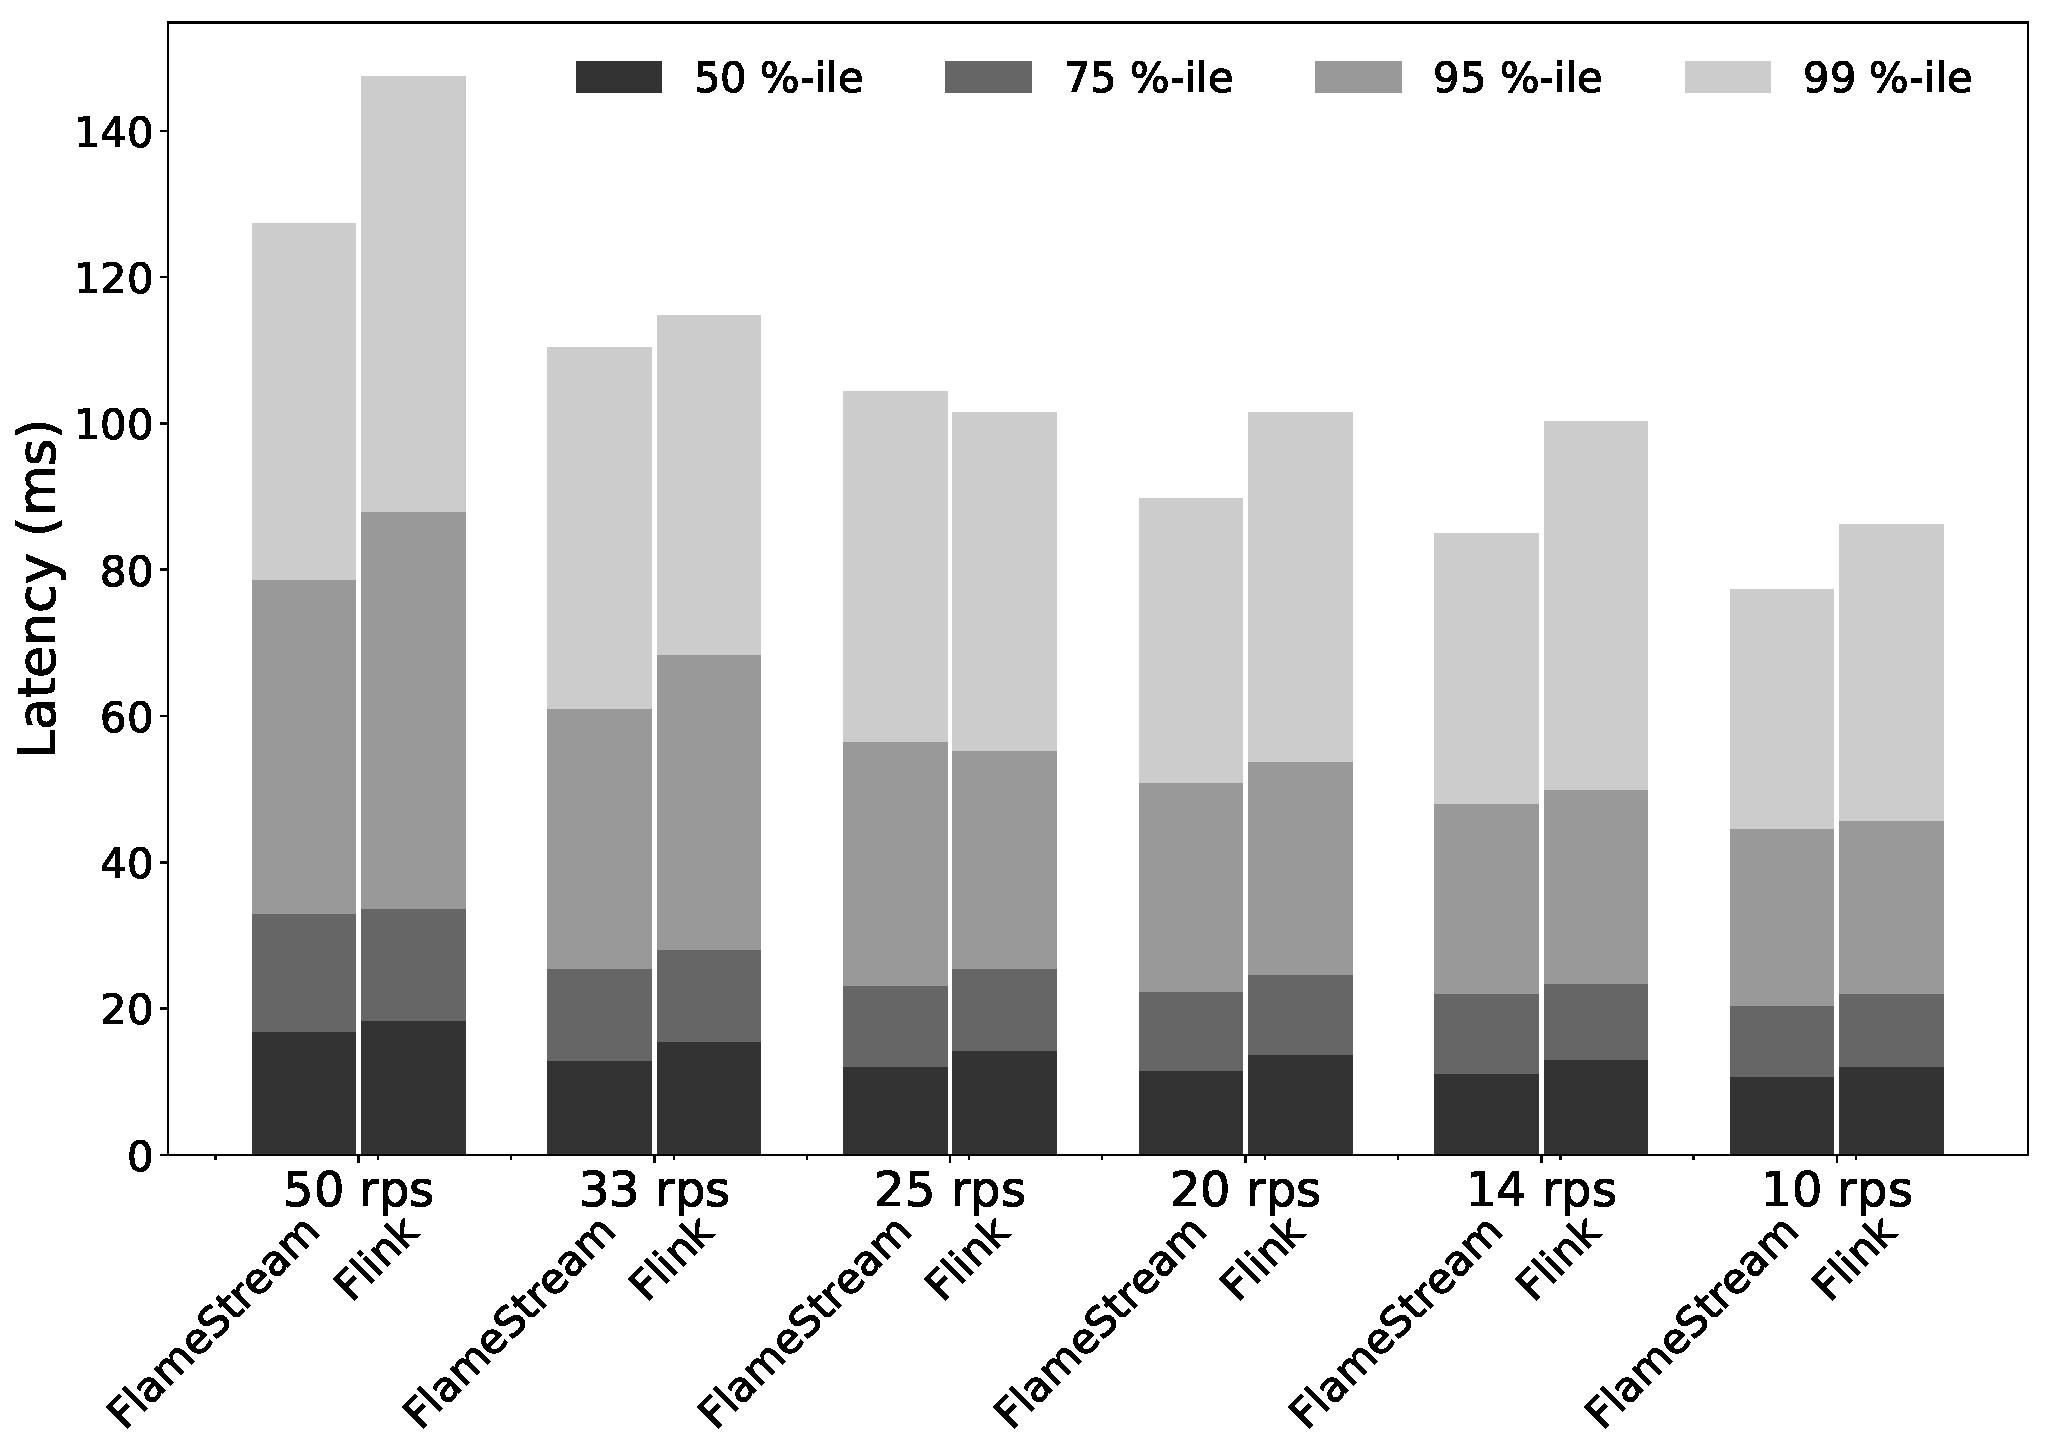
\includegraphics[width=\textwidth]{pics/comp-index-quantiles}
  \caption{The comparison in latencies between \FlameStream\ and Flink, (a) - 10 workers, (b) - 5 workers. (c) - the waiting time: Fling buffer vs. FlameStream barrier}
  \label {fs-index-quantiles}
\end{figure}

However, there are conditions, which are not suitable for the optimistic approach. The (b) plot in Figure~\ref{fs-index-quantiles} shows the comparison of latencies between \FlameStream\ and Flink within 5 nodes and distinct document rates. Flink outperforms \FlameStream\ under extreme load. Such behavior follows from the fact that \FlameStream\ provides significant overhead under very high pressure within a few computational units. This result evidently corresponds with measurements of the overhead in Figure~\ref{overhead}. Nevertheless, it should be noted that \FlameStream\ demonstrates better latency under non-extreme load.

Thus, Flink can be more appropriate if there is a need to optimize computational resources under a fixed load, but the demands on latency are not very strict, or determinism is not required. \FlameStream\ is more relevant for cases when low latency and determinism are strict requirements, but an allocation of additional resources is not a problem.  
